\documentclass[letterpaper,12pt,fleqn]{article}
\usepackage{matharticle}
\usepackage{tikz}
\pagestyle{plain}
\begin{document}
\section*{Rules}

We now are going to develop our mathematical system for what we can do with the
real numbers. We are going to establish a set of axioms for algebraic
manipulation of expressions and equations. Everything you do must be traceable
to these rules --- don't make things up!

\subsection*{Expressions}

\begin{definition}[Expression]
  An expression is a syntactic combination of constants, variables, and
  operators such that once values are selected for the variables, the
  expression can be evaluated using the rules of arithmetic to yield a single
  value.
\end{definition}

An expression, no matter how complicated, is just a number!

Arithmetic Precedence Rules:
\begin{enumerate}
\item $()$
\item Exponentiation (R to L)
\item Multiplication (L to R)
\item Addition (L to R)
\end{enumerate}

\begin{example}

  (Do this example by hand, and then using a calculator)
  
  $x+2^{x^y}-3(x+y)+y$

  Let $x=2$ and $y=3$
  \begin{eqnarray*}
    2+2^{2^3}-3(2+3)+3 &=& 2+2^8-3(5)+3 \\
    &=& 2+256-15+3 \\
    &=& 258-15+3 \\
    &=& 243+3 \\
    &=& 246 \\
  \end{eqnarray*}
\end{example}

Recursive Construction:
\begin{enumerate}
\item Constant
\item Variable
\item $(e)$
\item $e_1^{e_2}$
\item $f(x)$
\item $e_1e_2$ (products)
\item $e_1+e_2$ (terms)
\end{enumerate}

\bigskip

An important skill is the ability to identify the factors in an expression.

\begin{example}
  $(x+1)xy^2(z-1)$ has 4 factors: $(x+1), x, y^2, (z-1)$
\end{example}

From now on, a statement like $a\in\R$ should be taken to mean that $a$ is any
expression for a real number.

What matters in the final, evaluated value (point on the number line). Thus,
two expressions that result in the same value are said to be equal.

\begin{properties}[Equality]
  Let $a,b,c\in\R$:
  \begin{enumerate}
  \item Reflexive
    \[a=a\]
  \item Symmetric
    \[a=b\implies b=a\]
  \item Transitive
    \[a=b\ \mbox{and}\ b=c\implies a=c\]
  \end{enumerate}
\end{properties}

\begin{axiom}[Substitution Principle]
  If two algebraic expressions are equal then one can syntactically replace
  the other.
\end{axiom}

This is the basis for algebraic simplification: a simpler expression can
replace a more complicated expression when they are equal.

\begin{example}
  When $x=5$, $3x+1$ is replaced with $3(5)+1$ is replaced with $15+1$ is
  replaced with $16$.
\end{example}

And now, the 10 rules/axioms. Any mathematic system that follows these 10
axioms is called a field. Everything that we do is mathematical systems
involving the real numbers (including calculus) can be traced to one of these
original axioms.

(Ref: page 12)

Note: Closure of the binary operators is assumed.

\begin{properties}[Field Axioms]
  \listbreak
  \begin{enumerate}
  \item Commutative Addition (CA)
    \[\forall\,a,b\in\R,a+b=b+a\]
  \item Associative Addition (AA)
    \[\forall\,a,b,c\in\R,(a+b)+c=a+(b+c)\]
  \item Additive Identity (A0)
    \[\exists\,0\in\R,\forall\,a\in\R,a+0=0+a=a\]
  \item Additive Inverse (AI)
    \[\forall\,a\in\R,\exists\,-a\in\R,a+(-a)=(-a)+a=0\]
  \item Commutative Multiplication (CM)
    \[\forall\,a,b\in\R,ab=ba\]
  \item Associative Multiplication (AM)
    \[\forall\,a,b,c\in\R,(ab)c=a(bc)\]
  \item Multiplicative Identity (M1)
    \[\exists\,1\in\R,\forall\,a\in\R,a1=1a=a\]
  \item Multiplicative Inverse (MI)
    \[\forall\,a\in\R-\{0\},\exists\,a^{-1}\in\R,aa^{-1}=a^{-1}a=1\]
  \item Left Distributive (LD)
    \[\forall\,a,b,c\in\R,a(b+c)=ab+ac\]
  \item Right Distributive (LD)
    \[\forall\,a,b,c\in\R,(a+b)c=ac+bc\]
  \end{enumerate}
\end{properties}

Be careful not to mix the rules of addition and multiplication, and do not
make up rules of your own.

Because of commutativity and associativity, factors in products and products in
terms can be evaluated in any order --- but don't mix them!

\begin{example}
  $1+2(3)(5)+(-2)+3$
\end{example}

\begin{properties}[Zero]
  (Ref: page 14)
  \begin{enumerate}
  \item The additive identity is unique
  \item $-0=0$
  \item $\forall\,a\in\R,a0=0a=0$
  \item $\forall\,a,b\in\R,ab=0\implies a=0$ or $b=0$
  \end{enumerate}
\end{properties}

\begin{properties}[Negatives]
  (Ref: page 13)
  \begin{enumerate}
  \item Additive inverses are unique
  \item $-a=(-1)a$
  \item $-(-a)=a$
  \item $-(ab)=(-a)b=a(-b)$
  \item $(-a)(-b)=ab$
  \item $-(a+b)=(-a)+(-b)$
  \end{enumerate}
\end{properties}

Don't assume that $-a$ is a negative number when you don't know exactly what
$a$ is. For example, $a$ could be $-2$, in which case $-a=-(-2)=2$, which is
positive.

\begin{definition}[Subtraction]
  Subtraction is a syntactic convenience given by:
  \[a-b=a+(-b)\]
\end{definition}

Warnings about subtraction:
\begin{enumerate}
\item The negative sign applies to the syntactic element immediately
  following it:
  \[1-x+2=1+(-x)+2\]
  \[1-(x+2)=1-x-2\]
\item It does not follow the rules:
  \[2-1\ne1-2\]
  \[(2-3)-4\ne2-(3-4)\]
\item Be very careful with mixing subtraction and substitution:
  
  Let $y=x-5$
  
  $4-y=4-(x-5)=4-x+5=4+(-x)+5=9-x$
\end{enumerate}

\begin{definition}[Inverse]
  $\forall\,a\in\R-\{0\},a^{-1}=\frac{1}{a}$
\end{definition}

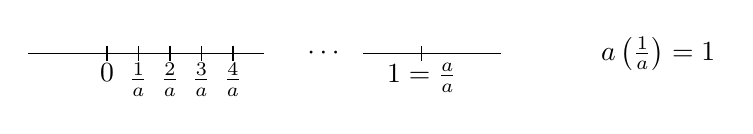
\begin{tikzpicture}
  \draw (-1,0) -- (2,0);
  \draw (3.25,0) -- (5,0);
  \draw (0,0.1) -- (0,-0.1);
  \draw (4/10,0.1) -- (4/10,-0.1);
  \draw (8/10,0.1) -- (8/10,-0.1);
  \draw (12/10,0.1) -- (12/10,-0.1);
  \draw (16/10,0.1) -- (16/10,-0.1);
  \draw (4,0.1) -- (4,-0.1);
  \node at (2.75,0) {$\cdots$};
  \node [below] at (0,0) {$0$};
  \node [below] at (4,0) {$1=\frac{a}{a}$};
  \node [below] at (4/10,0) {$\frac{1}{a}$};
  \node [below] at (8/10,0) {$\frac{2}{a}$};
  \node [below] at (12/10,0) {$\frac{3}{a}$};
  \node [below] at (16/10,0) {$\frac{4}{a}$};
  \node at (7,0) {$a\left(\frac{1}{a}\right)=1$};
\end{tikzpicture}

Don't assume that $a$ is simple; it may be a fraction as well:
  \[(a^{-1})^{-1}=\frac{1}{\frac{1}{a}}=a\]

\begin{definition}[Division]
  Division is a syntactic convenience given by:
  \[\frac{a}{b}=a\left(\frac{1}{b}\right)\]
\end{definition}

\begin{example}
  $\frac{a+b}{c}=\frac{1}{c}(a+b)=
  \left(\frac{1}{c}\right)a+\left(\frac{1}{c}\right)b=
  \frac{a}{c}+\frac{b}{c}$

  $\frac{a+b}{a}=\frac{1}{a}(a+b)=
  \left(\frac{1}{a}\right)a+\left(\frac{1}{a}\right)b=
  \frac{a}{a}+\frac{b}{a}=
  1+\frac{b}{a}$
\end{example}

\begin{example}
  How many factors are there in:
  \[\frac{(x+1)y^2}{z(w-1)^3}\]
  There are 4: $x-1, y^2, \frac{1}{z}, \frac{1}{(w-1)^3}$
  \[\frac{xy^2}{zw^3}=
  (x+1)(y^2)\left(\frac{1}{z}\right)\left[\frac{1}{(w-1)^3}\right]\]
\end{example}

\begin{properties}[Fractions]
  (Ref: page 14)

  $\forall\,a,b,c,d\in\R$ such that $b,d\ne0$:
  \begin{enumerate}
  \item $a\ne0\implies\frac{0}{a}=0$
  \item $\frac{a}{0}$ is undefined, or $\infty$, or indeterminate if $a=0$
  \item $\frac{a}{b}=\frac{c}{d}\iff ad=bc$
  \item $-\frac{a}{b}=\frac{-a}{b}=\frac{a}{-b}$
  \item $\frac{-a}{-b}=\frac{a}{b}$
  \item $c\ne0\implies\frac{a}{b}=\frac{ac}{bc}$
  \item $\frac{a}{b}\pm\frac{c}{b}=\frac{a\pm c}{b}$
  \item $\frac{a}{b}\pm\frac{c}{d}=\frac{ad\pm bc}{db}$
  \item $\left(\frac{a}{b}\right)\left(\frac{c}{d}\right)=\frac{ac}{bd}$
  \item $c\ne0\implies\left(\frac{a}{b}\right)\div\left(\frac{c}{d}\right)=
    \frac{\frac{a}{b}}{\frac{c}{d}}=
    \left(\frac{a}{b}\right)\left(\frac{d}{c}\right)=
    \frac{ad}{bc}$
  \end{enumerate}
\end{properties}

\end{document}
